%\chapter{Ferramentas do Projeto}

\chapter{ALGORITMOS DE APRENDIZADO DE MÁQUINAS}

As técnicas de aprendizagem de máquinas surgiram da necessidade de otimização de detecção de padrões não explícitos. Dentre as diferentes aplicações no mercado de trabalho, existe a detecção de fraudes, analise de currículo e Previsão de falha de equipamentos, por exemplo em 
\cite{santander}.

Oito algoritmos foram escolhidos para realização dos testes. Cada um desses algoritmos é descrito neste capítulo, com suas principais vantagens e desvantagens.

\section{\textbf{Supervisionada}}
Na aprendizagem supervisionada treinamos os algoritmos utilizados, dados que já temos o gabarito, ou seja, já foram mapeados com as saídas desejadas. O algoritmos deverá ter a capacidade de se treinar e comparar o resultado previsto com o idealizado. 

Problemas de aprendizagem supervisionada são classificados em problemas de “regressão” e “classificação”. Em um problema de regressão, objetiva-se prever os resultados em uma saída contínua, o que significa que é desejado mapear variáveis de entrada para alguma função contínua. Em um problema de classificação, objetiva-se prever os resultados em uma saída discreta, isto é, o objetivo é mapear variáveis de entrada em categorias distintas\cite{aprendizagem}.

Exemplo:
 \renewcommand{\theenumi}{\Alph{enumi}}
 \begin{enumerate}
 
    \item Regressão - Dada uma imagem de homem/mulher, temos de prever sua idade com base em dados da imagem.
    \item Classificação - Dada um exemplo de tumor cancerígeno, temos de prever se ele é benigno ou maligno através do seu tamanho e idade do paciente.
     
 \end{enumerate}


Foram usado diferentes algoritmos para determinar aquele com melhor eficácia para o sistema. 
\subsection{{Classificador por Árvore de decisão}}

A árvore de classificação é o resultado de se fazer uma sequência ordenada de perguntas, e as perguntas feitas a cada passo na sequência dependem das respostas às perguntas anteriores. A sequência termina em uma previsão da classe.
O ponto de partida de uma árvore de classificação é chamado de nó raiz e consiste em todo o conjunto de aprendizado, e está no topo da árvore. Um nó é um subconjunto do conjunto de atributos, e pode ser terminal ou não-terminal. Um nó não-terminal é um nó que se divide em nós filhos. Tal divisão é determinada por uma condição sobre o valor de um único atributo, e que vai dividir os exemplos de acordo com a condição, em outros nós. Um nó que não se divide é chamado de nó terminal, e a ele é atribuída uma classe. Cada exemplo no conjunto cai em um dos nós terminais. 

Uma árvore de decisão é um mapa dos possíveis resultados de uma série de escolhas relacionadas. Geralmente começa com um único nó, que se divide em possíveis resultados. Cada um desses resultados leva a nós adicionais, que se ramificam em outras possibilidades. Assim, cria-se uma forma de árvore. Tem alta taxa de compreensão dos dados, mas podem se tornar excessivamente complexas e por consequência pesadas. A \ref{fig:arvoredecisao} mostra de forma simplificada como é feita essa categorização. 


\begin{figure}[H]
\begin{center}
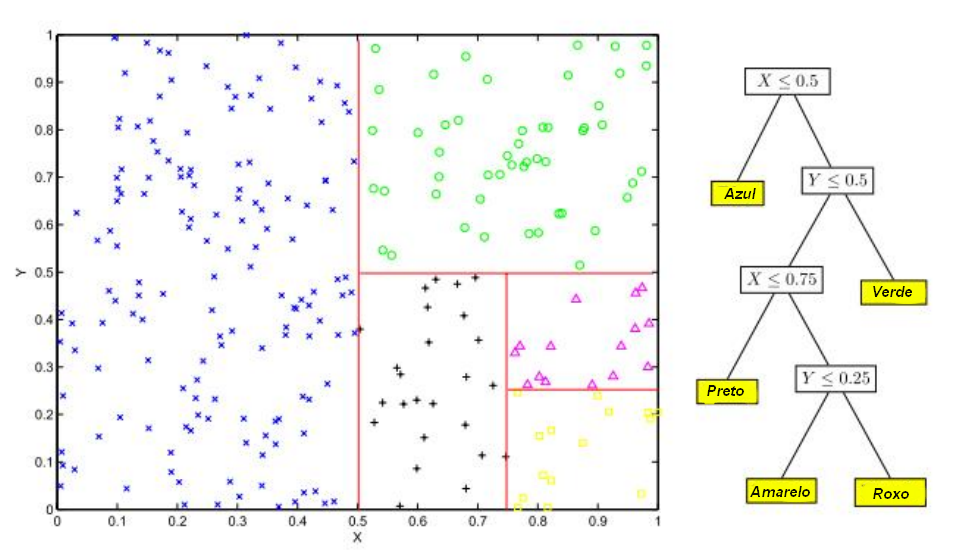
\includegraphics[width=13cm]{./02_Cap2/figures/arvore_de_decisao.png}
\caption{\label{fig:arvoredecisao}- Exemplo de partições em árvores de decisão.}
\end{center}
\end{figure}

O processo de crescimento de uma árvore de classificação necessita responder a quatro questões básicas: Como escolher as condições para dividir cada nó? Que critério devemos usar para dividir um nó pai em seus nós filhos? Como vamos decidir quando um nó se tornará um nó terminal (parar a divisão)? Como vamos atribuir uma classe a esse nó terminal?

Existe uma série de equações que ajudam o algorítimo a responder às perguntas levantadas. A principal delas é a de entropia que caracteriza a impureza dos dados, num conjunto, ela caracteriza a falta de homogeneidade dos dados de entrada em relação à sua classificação. Por exemplo, a entropia é máxima (igual a 1) quando o conjunto de dados é heterogêneo e miníma (igual a 0) quando os dados são totalmente homogêneos. Dado um conjunto de entrada S que pode ter c classes distintas e tendo pi o identificador de quantos de dados em S que pertence a classe i. a entropia de S será dada por:
\begin{equation}
E(S) = \sum_{i=1}^{c}-pi*log(pi)
\end{equation}
Utilizando essa equação, o código consegue saber se os dados estão homogêneos e se deve ou não criar novos nós de decisão\cite{arvored}. 




\subsection{{Classificador AdaBoost}}

O AdaBoost é um algoritmo de aprendizado supervisionado do tipo boost. Seu nome deriva de Adaptive Boosting, no sentido que ele é adaptado através de um sistema de pesos durante sua execução.O AdaBoost combina um conjunto de funções simples de classificação, denominadas classificadores fracos (como a arvore de decisão) para formar um classificador forte. 
Um classificador forte é composto de um conjunto de classificadores fracos, associados
a pesos que classificam de forma precisa dois conjuntos de dados pré-rotulados, onde as
características com pesos maiores são mais significativas para a classificação de exemplos definidos como parte de um certo conjunto. Na Equação a seguir é formalizada a criação de um classificador forte através de um algoritmo de Boosting.
\begin{equation}
H(x) = α1h1 + α2h2 + ... + αnhn(x)
\end{equation}
onde \[H(x)\] é um classificador forte, αi é o peso associado ao classificador hi. 
Dado uma base de dados de entrada, a função do AdaBoost é encontrar o conjunto de características que comporão o classificador forte provendo uma melhor classificação do conjunto de entrada\cite{AdaBoost}.




\subsection{{Classificador Floresta aleatória}}

Floresta Aleatória (Random Forest) é um algoritmo de aprendizagem de máquina flexível que produz excelentes resultados a maioria das vezes, mesmo sem ajuste de hiperparâmetros. É também um dos algoritmos mais utilizados, devido à sua simplicidade e o fato de que pode ser utilizado para tarefas de classificação e também de regressão. 

O algoritmo cria uma floresta de um modo aleatório. A “floresta” criada é uma combinação de árvores de decisão como demostra a \ref{fig:randomfloresta}, na maioria dos casos treinados com o método de bagging ( estimador aleatório). A idéia principal do método de bagging é que a combinação dos modelos de aprendizado aumenta o resultado geral.


\begin{figure}[H]
\begin{center}
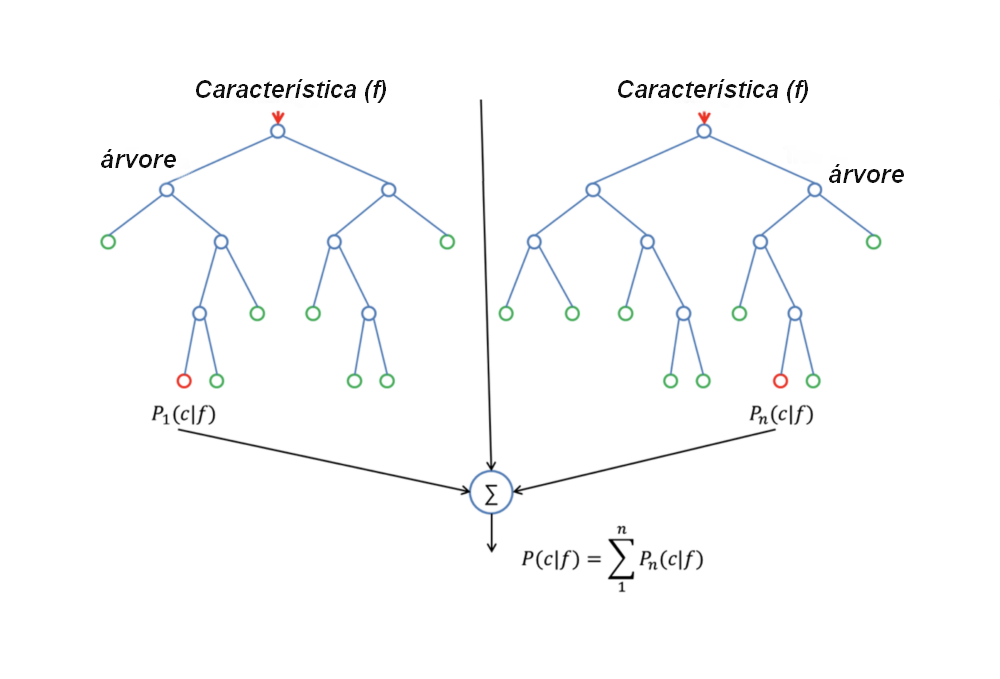
\includegraphics[width=13cm]{./02_Cap2/figures/forestRandom.png}
\caption{\label{fig:randomfloresta}- Floresta aleatória.}
\end{center}
\end{figure}



 A floresta aleatória adiciona aleatoriedade extra ao modelo, quando está criando as árvores. Ao invés de procurar pela melhor característica ao fazer a partição, ele busca a melhor característica em um subconjunto aleatório das características. Este processo cria uma grande diversidade, o que geralmente leva a geração de modelos melhores.

Uma grande vantagem do algoritmo de florestas aleatórias é que ele pode ser utilizado tanto para tarefas de classificação quanto para regressão, o que representa a maioria dos sistemas de aprendizagem de máquina atuais.

Outra grande qualidade das florestas aleatórias é a facilidade para se medir a importância relativa de cada característica para a predição. É possível medir  a relevância das características analisando quantos nodos das árvores, que usam uma dada característica, reduzem impureza geral da floresta, ou seja, aumenta a precisão da decisão não deixando a predição ser alterada por ruídos. Ele calcula este valor automaticamente para cada característica após o treinamento e normaliza os resultados para que a soma de todas as importâncias seja igual a 1. Isso ajuda a escolher quais variáveis utilizadas estão realmente influenciando nos dados finais\cite{Floresta}. 


\subsection{{Classificador Gaussiano de Naive Bayes}}

O algoritmo Naive Bayes é um classificador probabilístico baseado no “Teorema de Bayes”, o qual foi criado por Thomas Bayes (1701 - 1761) para tentar provar a existência de Deus.
Tornou-se popular na área de Aprendizado de Máquina para categorizar textos baseado na frequência das palavras usadas, e assim pode ser usado para identificar se determinado e-mail é um SPAM ou sobre qual assunto se refere determinado texto, por exemplo.

É matematicamente muito simples e rápido comparado a outros classificadores. Além disso, o Naive Bayes só precisa de um pequeno número de dados de teste para concluir classificações com uma boa precisão\cite{Bayes}.

 Sua característica marcante é ele desconsiderar completamente a correlação entre as variáveis. Dessa Forma cada variável é tratado, cada um, de forma independente entre si.  

O algoritmo de Naive Bayes consiste em encontrar a probabilidade Futura multiplicando a probabilidade inicial dado a probabilidade condicional, conforme a equação a seguir \cite{Bayes2}. 
\begin{equation}
P(A\mid B )= \frac{P(B\mid A )*P(A)}{P(A)}
\end{equation}


\subsection{{Classificador K vizinhos mais próximos}}

A ideia principal do KNN é determinar o rótulo de classificação de uma amostra baseado nas amostras vizinhas advindas de um conjunto de treinamento. Na \ref{fig:knn} é exemplificada uma aplicação, na qual temos um problema de classificação com dois rótulos de classe e com k = 7. No exemplo, são aferidas as distâncias de uma nova amostra, representada por uma estrela, às demais amostras de treinamento, representadas pelos circulos azuis e amarelas. A variável k representa a quantidade de vizinhos mais próximos que serão utilizados para averiguar a qual classe a nova amostra pertence. Com isso, das sete amostras de treinamento mais próximas da nova amostra, 4 são do rótulo A e 3 do rótulo B. Portanto, como existem mais vizinhos do rótulo A, a nova amostra receberá o mesmo rótulo deles, ou seja, A.

\begin{figure}[H]
\begin{center}
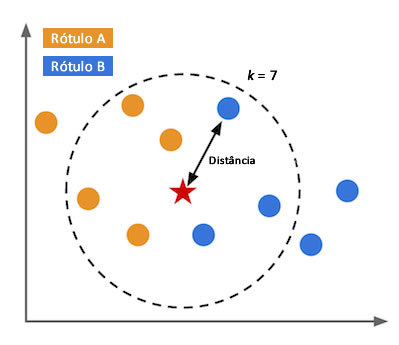
\includegraphics[width=7cm]{./02_Cap2/figures/imgKnn.png}
\caption{\label{fig:knn}- classificação do KNN com dois rótulos de classe e k = 7.}
\end{center}
\end{figure}

Dois pontos chaves que devem ser determinados para aplicação do KNN são: a métrica de distância e o valor de k. Para métrica de distância a mais utilizada é a distância Euclidiana, descrita na equação a seguir.
\begin{equation}
 D = \sqrt{(p_1 - q_1)^2 + \cdots + (p_n - q_n)^2} = \sqrt{\sum_{i=1}^n (p_i - q_i)^2}
 \end{equation}

onde $$P = (p_1, \cdots, p_n)$$  e $$Q = (q_1, \cdots, q_n)$$ são dois pontos n -dimensionais. 

A grande vantagem do KNN é sua abordagem simples de ser compreendida e implementada. Todavia, calcular distância é tarefa custosa e caso o problema possua grande número de amostras o algoritmo pode consumir muito tempo computacional. Além disso, o método é sensível à escolha do k que não possui um valor estabelecido, será variável com os dados\cite{knn}. 



\subsection{{Classificador Gradiente de descida estocástica}}

A Descida do Gradiente é uma ferramenta padrão para otimizar funções complexas iterativamente dentro de um programa de computador. Seu objetivo é encontrar um mínimo. Para as funções mais complexas pode haver muitos mínimos, a função de uma otimização seria encontrar o melhor mínimo. 

A Descida do Gradiente pode ser lenta para executar em conjuntos de dados muito grandes. Como uma iteração do algoritmo de descida do gradiente requer uma previsão para cada instância no conjunto de dados de treinamento, pode demorar muito quando existe milhares de instâncias.

Em situações em que se possui grandes quantidades de dados, você pode usar uma variação da descida do gradiente chamada Gradiente de descida estocástica.

Nesta variação, o procedimento de descida do gradiente é executado, mas a atualização para os coeficientes é realizada para cada instância de treinamento, em vez do final do lote de instâncias.

O primeiro passo do procedimento exige que a ordem do conjunto de dados de treinamento seja aleatória. Isto é, misturar a ordem que as atualizações são feitas para os coeficientes. Como os coeficientes são atualizados após cada instância de treinamento, as atualizações serão intensas, e assim o custo correspondente funcionará. Ao misturar a ordem para as atualizações dos coeficientes, ela aproveita essa caminhada aleatória e evita que ela fique “distraída” ou presa.

O procedimento de atualização para os coeficientes é o mesmo que o anterior, exceto que o custo não é somado em todos os padrões de treinamento, mas sim calculado para um padrão de treinamento.

A aprendizagem pode ser muito mais rápida com descida de gradiente estocástica para conjuntos de dados de treinamento muito grandes e muitas vezes apenas se precisa de um pequeno número de passagens através do conjunto de dados para alcançar um conjunto de coeficientes bom o suficiente \cite{gradiente}.



\subsection{{Classificador de Regressão logística}}

A regressão logística pode ser definida como um tipo de análise de regressão
muito semelhante a regressão linear. A diferença sutil entre os dois modelos é que
enquanto na regressão linear temos um valor real como saída, na regressão logística
temos um resultado binário. Ou seja, a partir de um determinado valor a saída torna-se “0” e no contrário temos um valor “1”. Dentre diversas aplicações, a mais direta é para o uso de classificação. 

É útil para modelar a probabilidade de um evento ocorrer como função de outros fatores.
 regressão logística analisa dados distribuídos binominalmente da forma:
 
\begin{equation}
     Y_{i}\ \sim B(p_{i},n_{i}),{\text{ for }}i=1,\dots ,m,
\end{equation}
Onde os números de ensaios de Bernoulli ni são conhecidos e as probabilidades de êxito pi são desconhecidas. O modelo é então obtido na base de que cada ensaio (valor de i) e o conjunto de variáveis explicativas/independentes possa informar acerca da probabilidade final \cite{logistica}.

\subsection{{Classificador Máquinas de vetores de suporte}}

Os fundamentos de SVM são provenientes da Teoria de Aprendizagem Estatística desenvolvida
inicialmente pelo pesquisador russo Vladmir Vapnik e colaboradores \cite{Vanpick} que idealizaram o princípio indutivo de Minimização do Risco Estrutural.

Embora as pesquisas desenvolvidas com SVM sejam recentes, as raízes do método foram
formuladas na década de 70. Inicialmente o método tinha dois problemas que foram resolvidos na década de 90 que iniciaram uma era de pesquisas com esse método.  
Essa aplicação categoriza as classes reconhecendo suas diferenças, assim podemos obter um padrão complexo dos dados mesmo sem ter um conhecimento prévio acerca do comportamento. Dessa forma, ele funciona de maneira similar a uma caixa preta, recebendo entradas e gerando uma saída que pode ser muito útil para encontrar padrões em dados que são muito complexos e não óbvios.

Uma das melhores características das máquinas de vetores de suporte é que elas são capazes de lidar muito bem com erros e ruídos nos dados. Elas são geralmente capazes de perceber o padrão de fundo nos dados e filtrar valores de dados atípicos e outras complexidades \cite{MetaQuotes}.







